
\section*{\centering{DVCS analysis update for EG6 meeting}}

\subsection*{\centering{Tuning the $^{4}He$ track parameters}}
- After the first and the second round comments, the $^{4}He$ track parameters 
have been tuned by looking at these parameters after the DVCS exclusivity 
cuts.\\
- In figure \ref{fig:He_pid_cuts}, I list the $^{4}He$ DVCS track parameters 
with the updated cuts.\\
- These cuts were applied to the following two analysis sets, except sdist cut 
on the old analysis set was [-3:3].\\

\begin{figure}[h!]
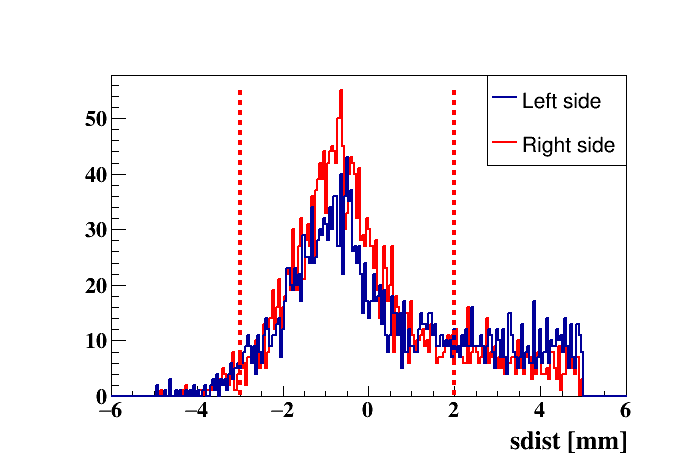
\includegraphics[height=6.0cm]{new_plots/rtpc_sdist.png}
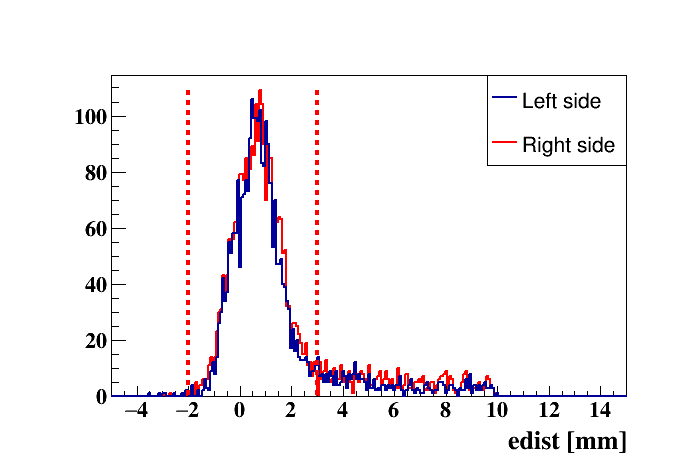
\includegraphics[height=6.0cm]{new_plots/after_rtpc_edist.png}
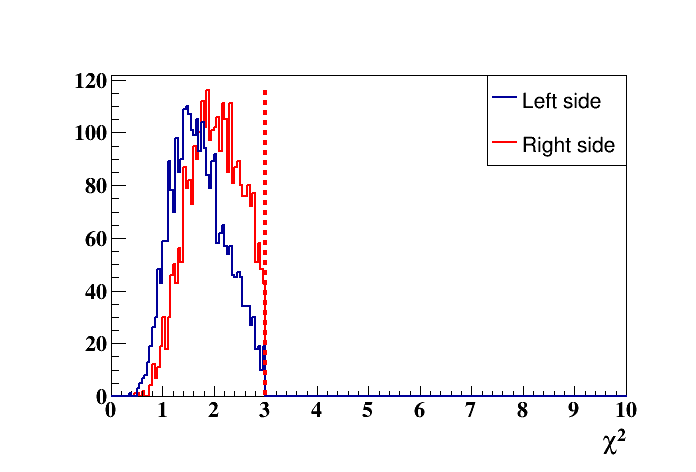
\includegraphics[height=6.0cm]{new_plots/after_rtpc_X2.png}
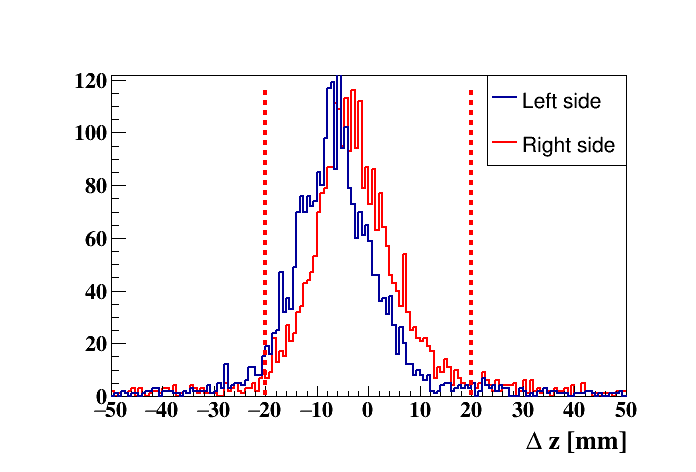
\includegraphics[height=6.0cm]{new_plots/after_rtpc_delta_z.png}
\caption{The distributions of the $^{4}He$ DVCS track parameters after applying 
the exclusivity cuts with the final cuts.}
\label{fig:He_pid_cuts}
\end{figure}






\subsection*{\centering{Exclusive distributions and reconstructed $A_{LU}$}}
After the suggestion from the review committee, I have changed the cut one the 
missing energy to be from [-0.45, 0.5] instead of a 3$\sigma$ cut on the 
distribution and refined all the other exclusive cuts. Figure 
\ref{fig:exc_cuts} presents the old and the new distributions for the exclusive 
variables.\\

- Note in the following plots, I will label the two analysis sets as "old", 3 
sigma cuts on all the variables, and "new", with the new missing energy cut and 
the corresponding updated 3 sigma cuts on the other variables.



\begin{figure}[h!]
\centering
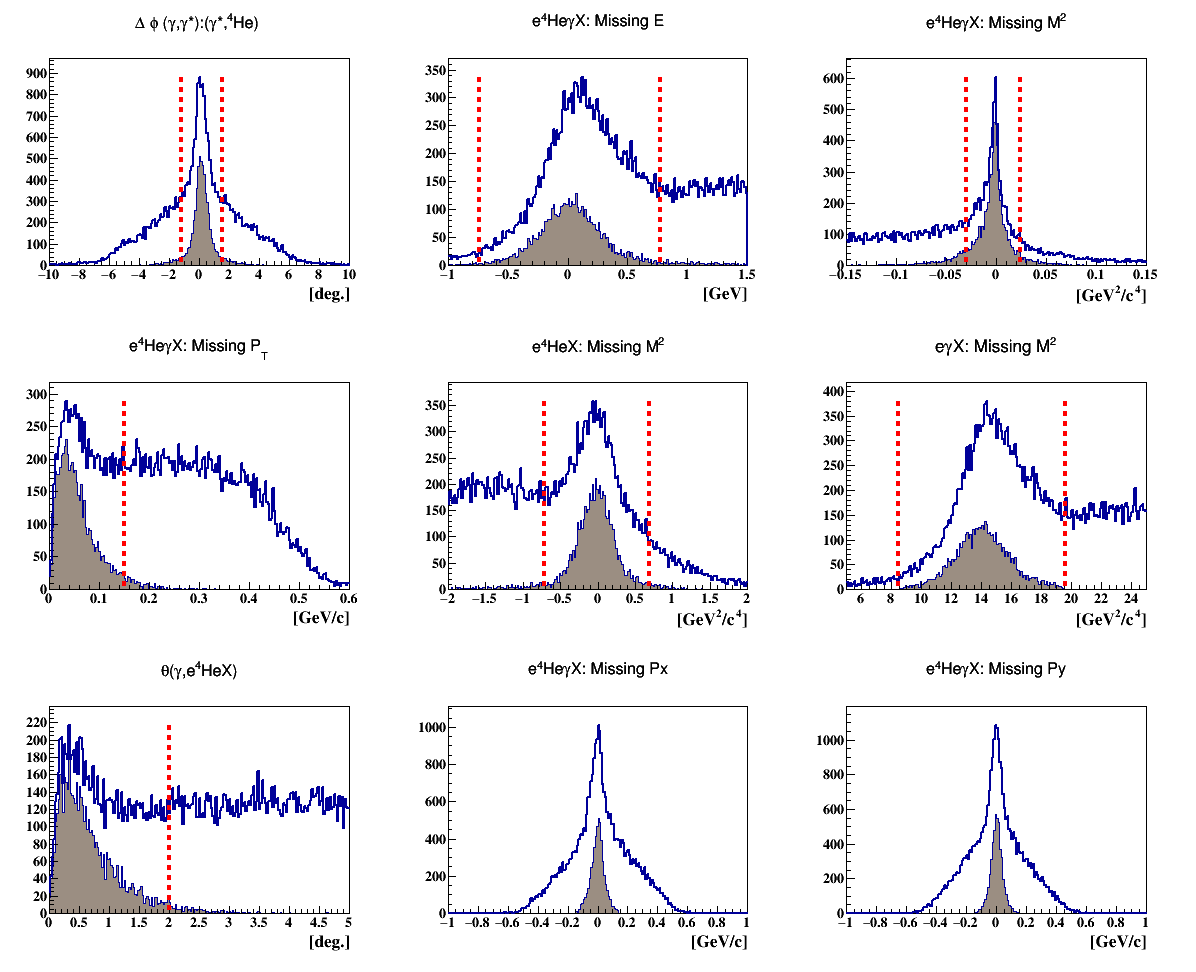
\includegraphics[height=10.0cm]{old_plots/all_coh_exc_cuts.png}
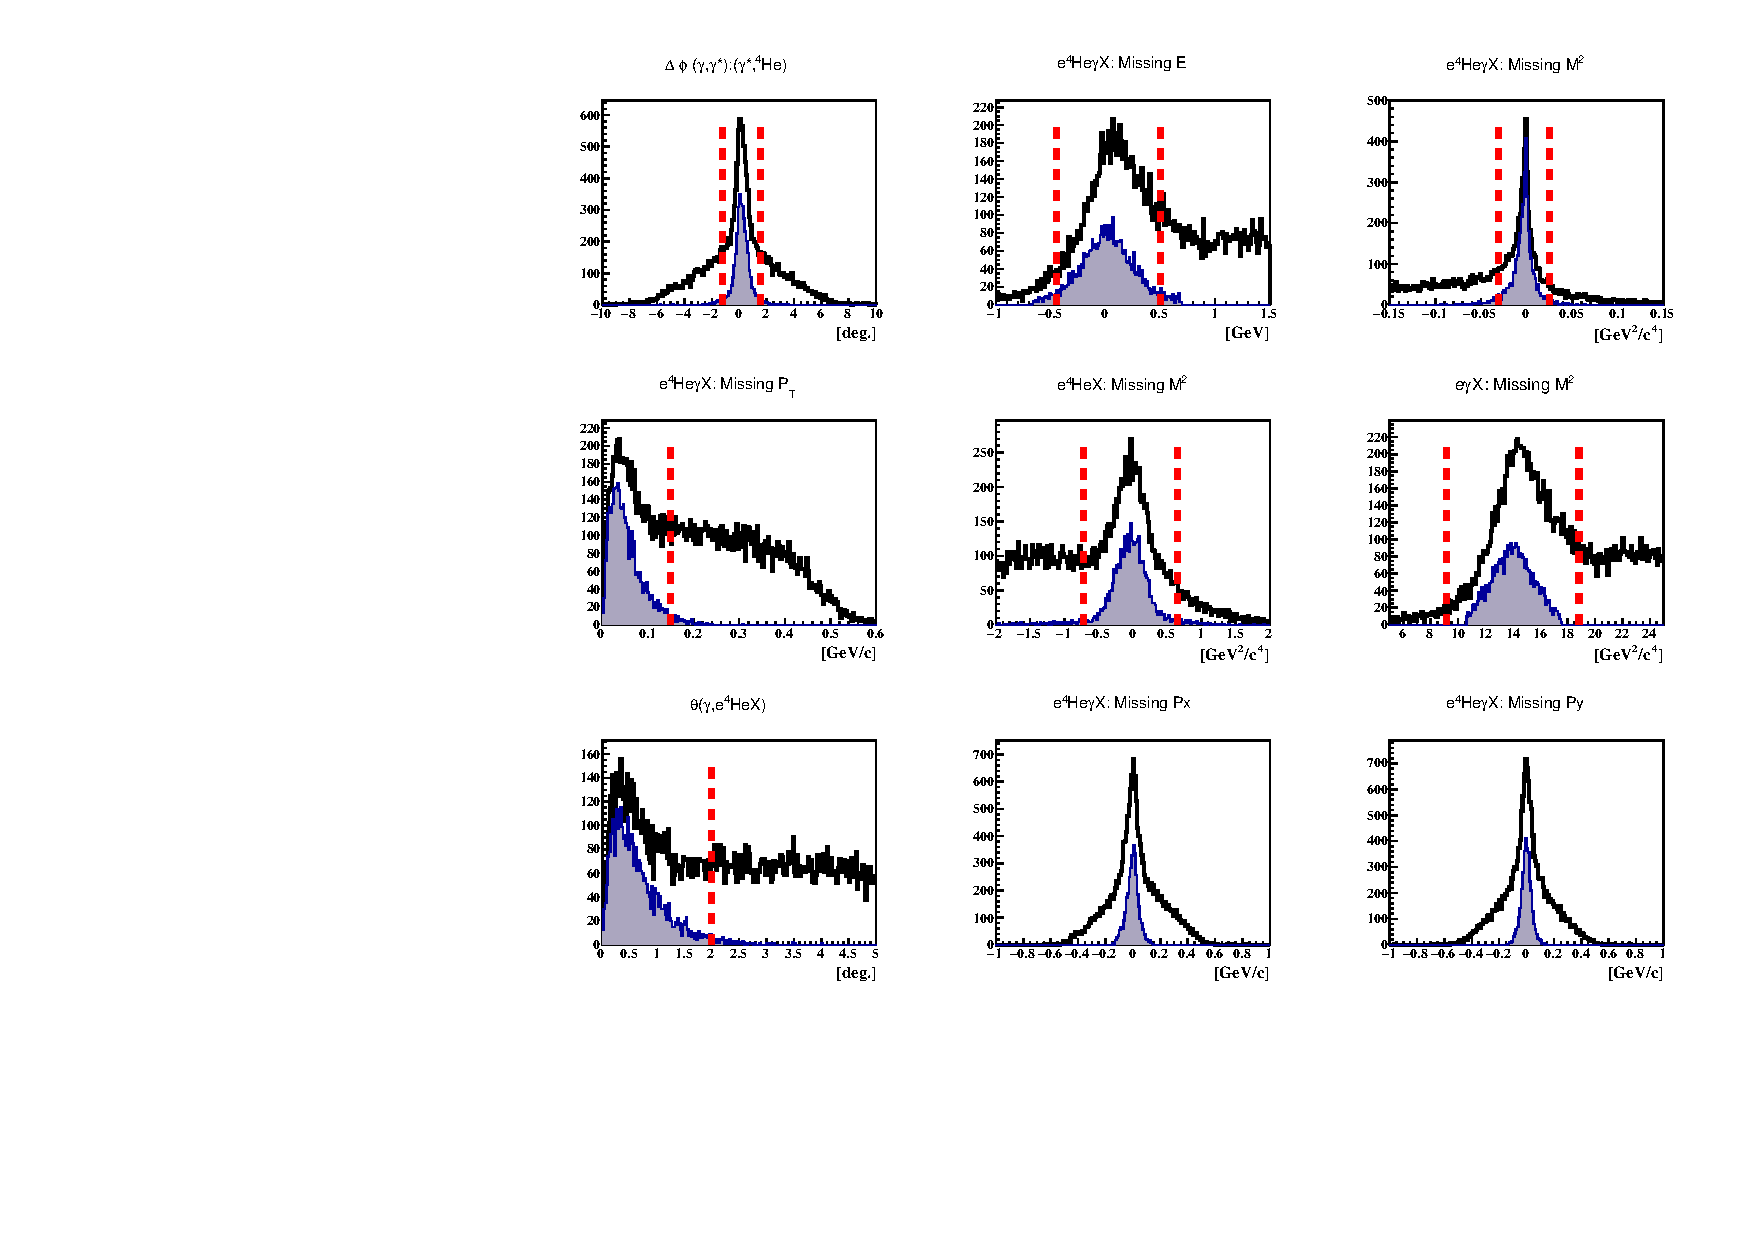
\includegraphics[height=10.0cm]{new_plots/all_coh_exc_cuts.pdf}
\caption{ }
\label{fig:exc_cuts}
\end{figure}



\begin{figure}[h!]
\centering
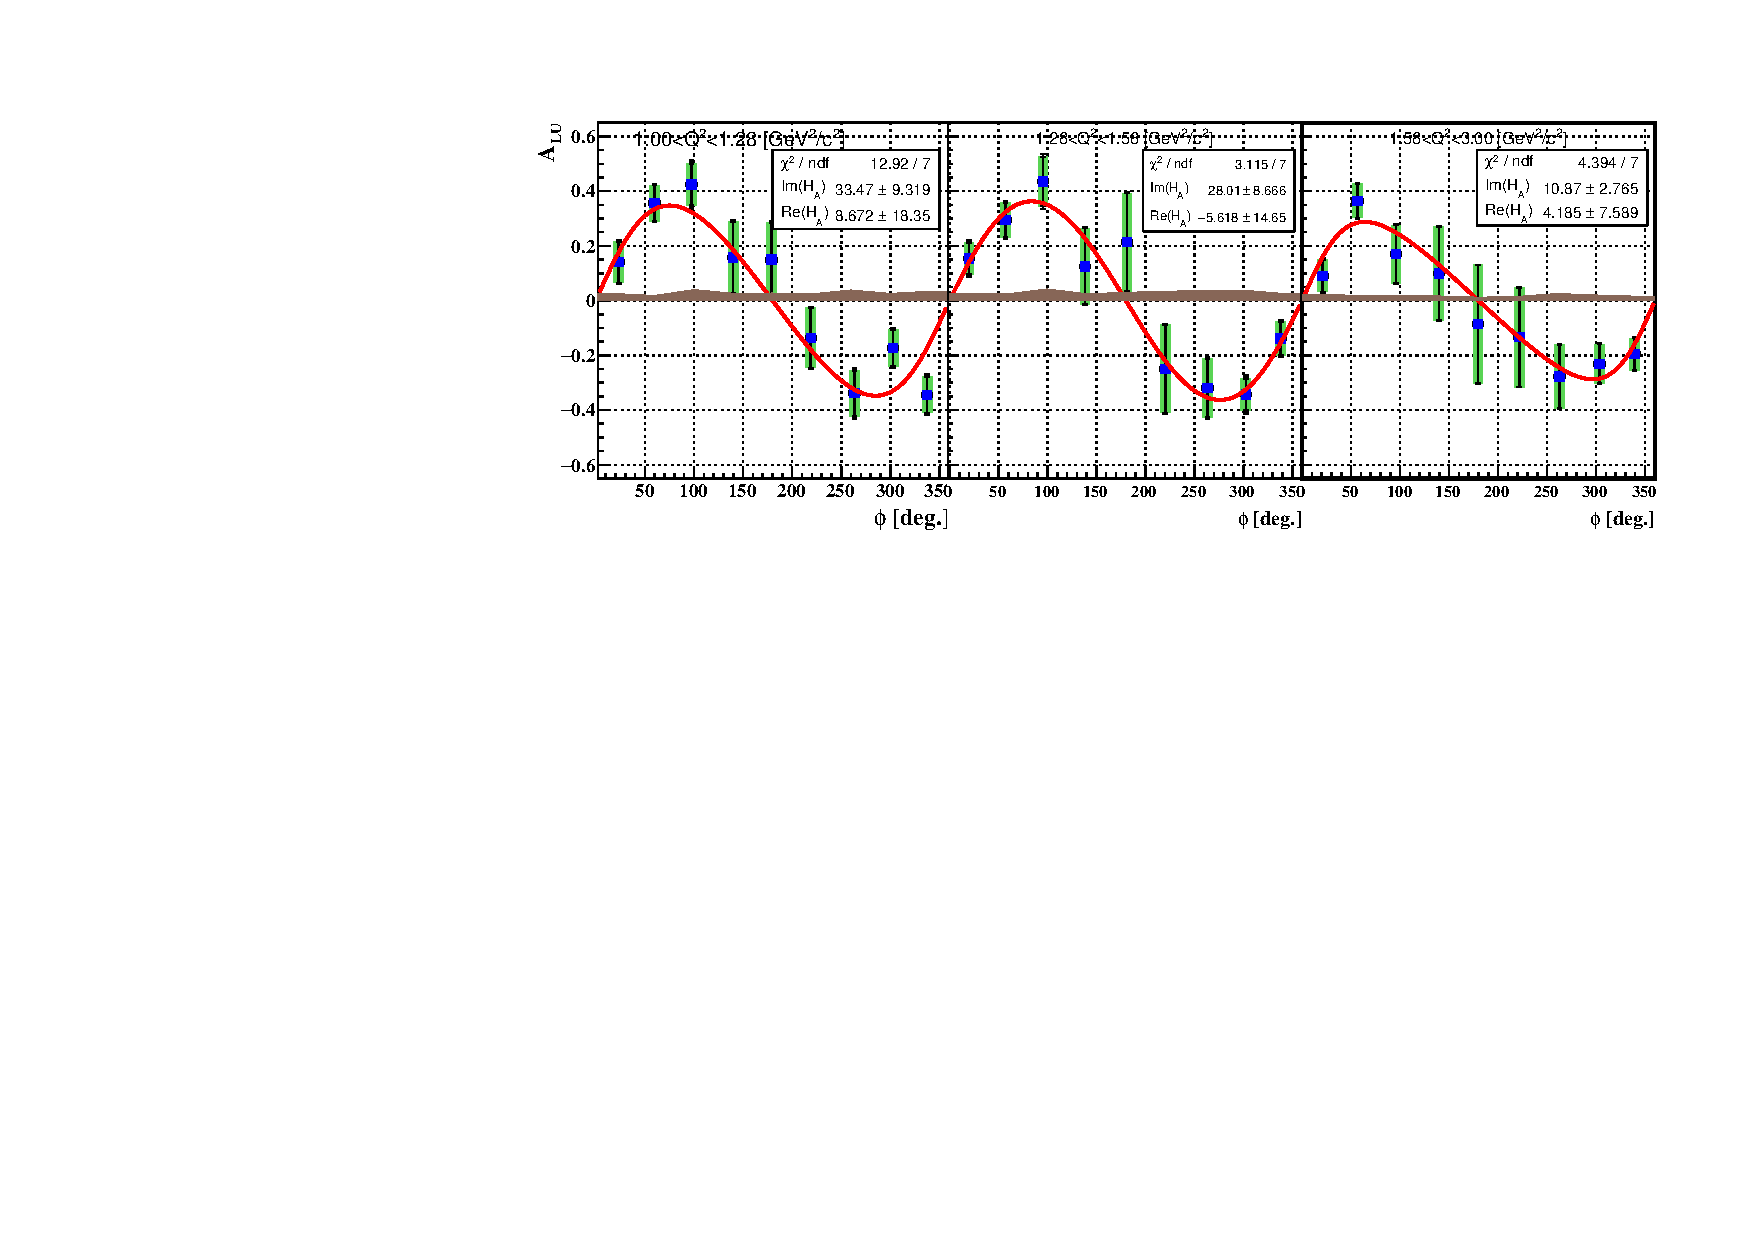
\includegraphics[height=7.5cm]{old_plots/f_coh_alu_Q2_phi.pdf}
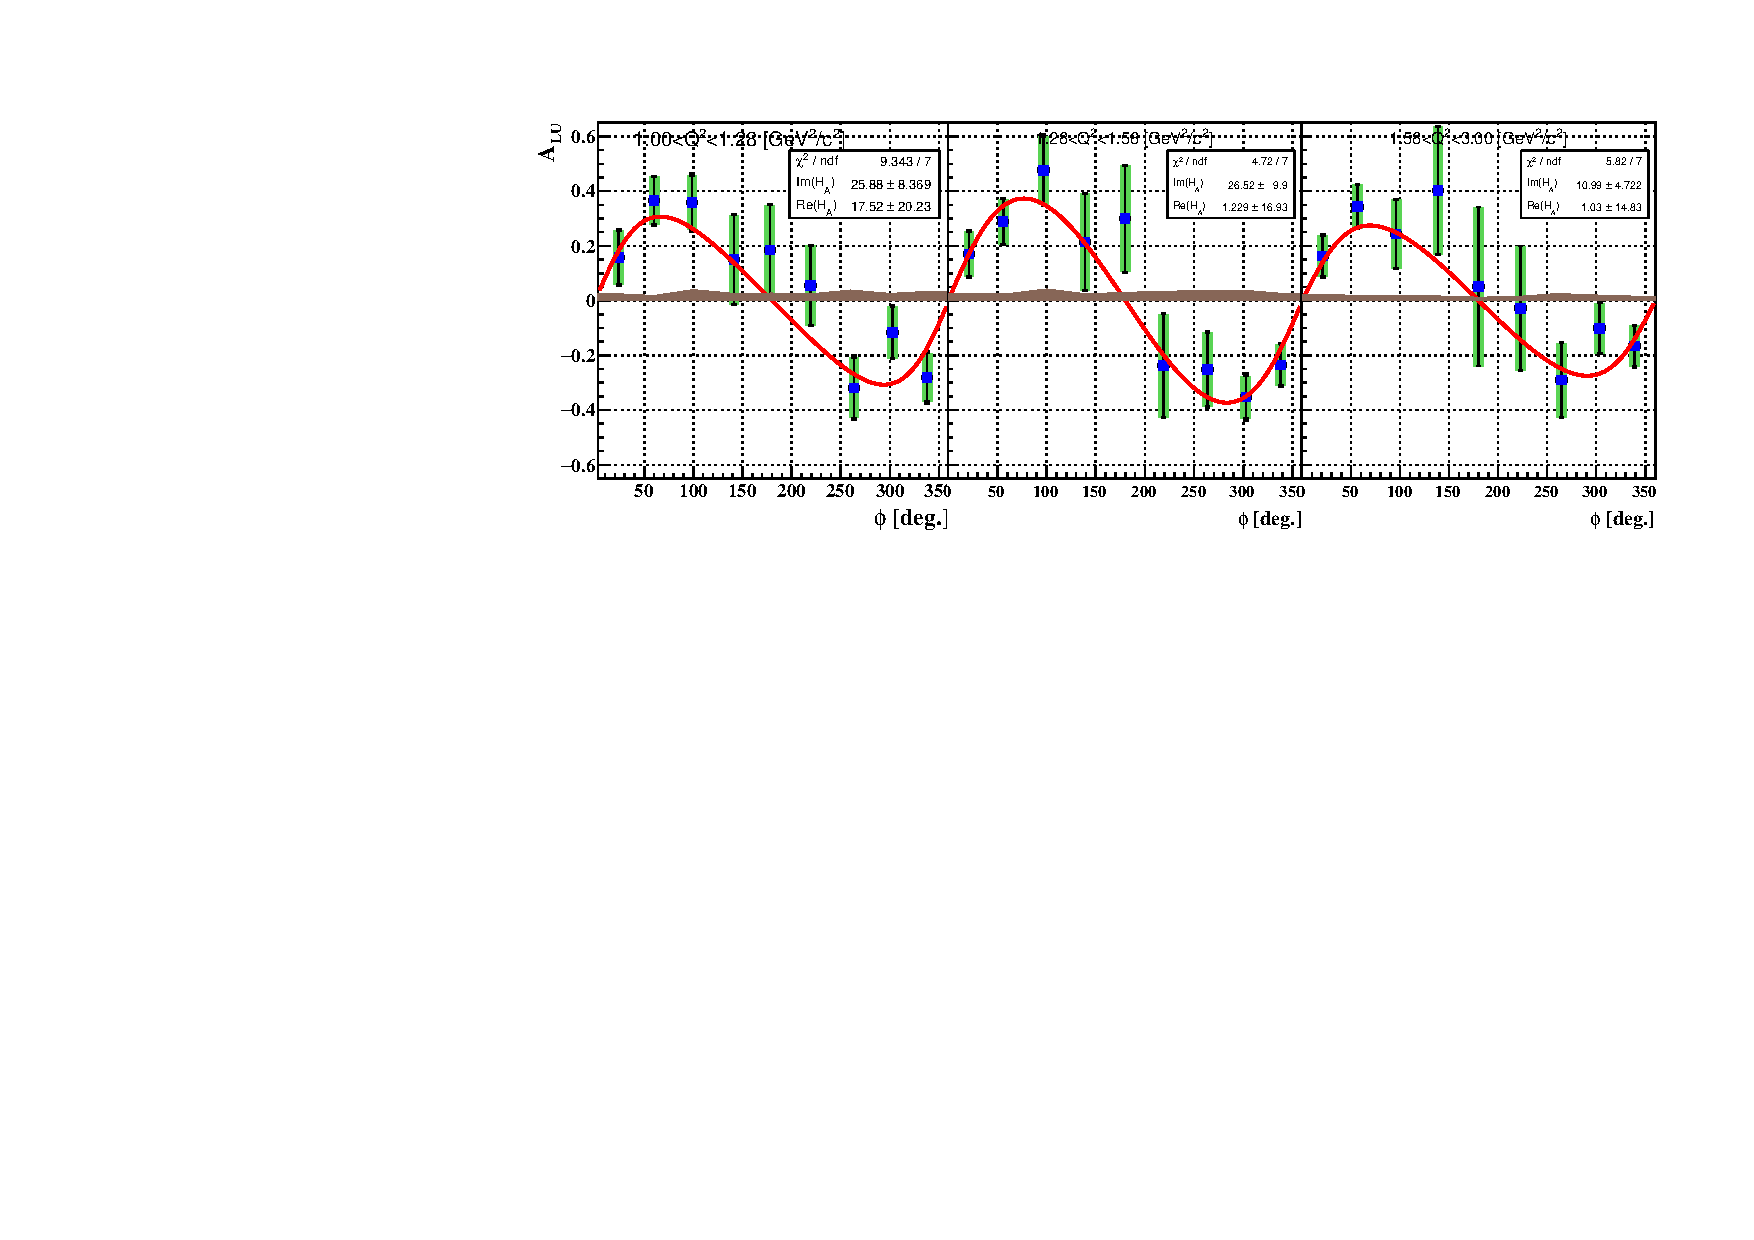
\includegraphics[height=7.5cm]{new_plots/Coh_ALU_Q2_phi.pdf}
\caption{Coherent $A_{LU}$ as a function of $\phi$ in $Q^{2}$ bins for old 
(top) and new (bottom) selection sets.}
\label{fig:ALU_Q2_phi}
\end{figure}


\begin{figure}[h!]
\centering
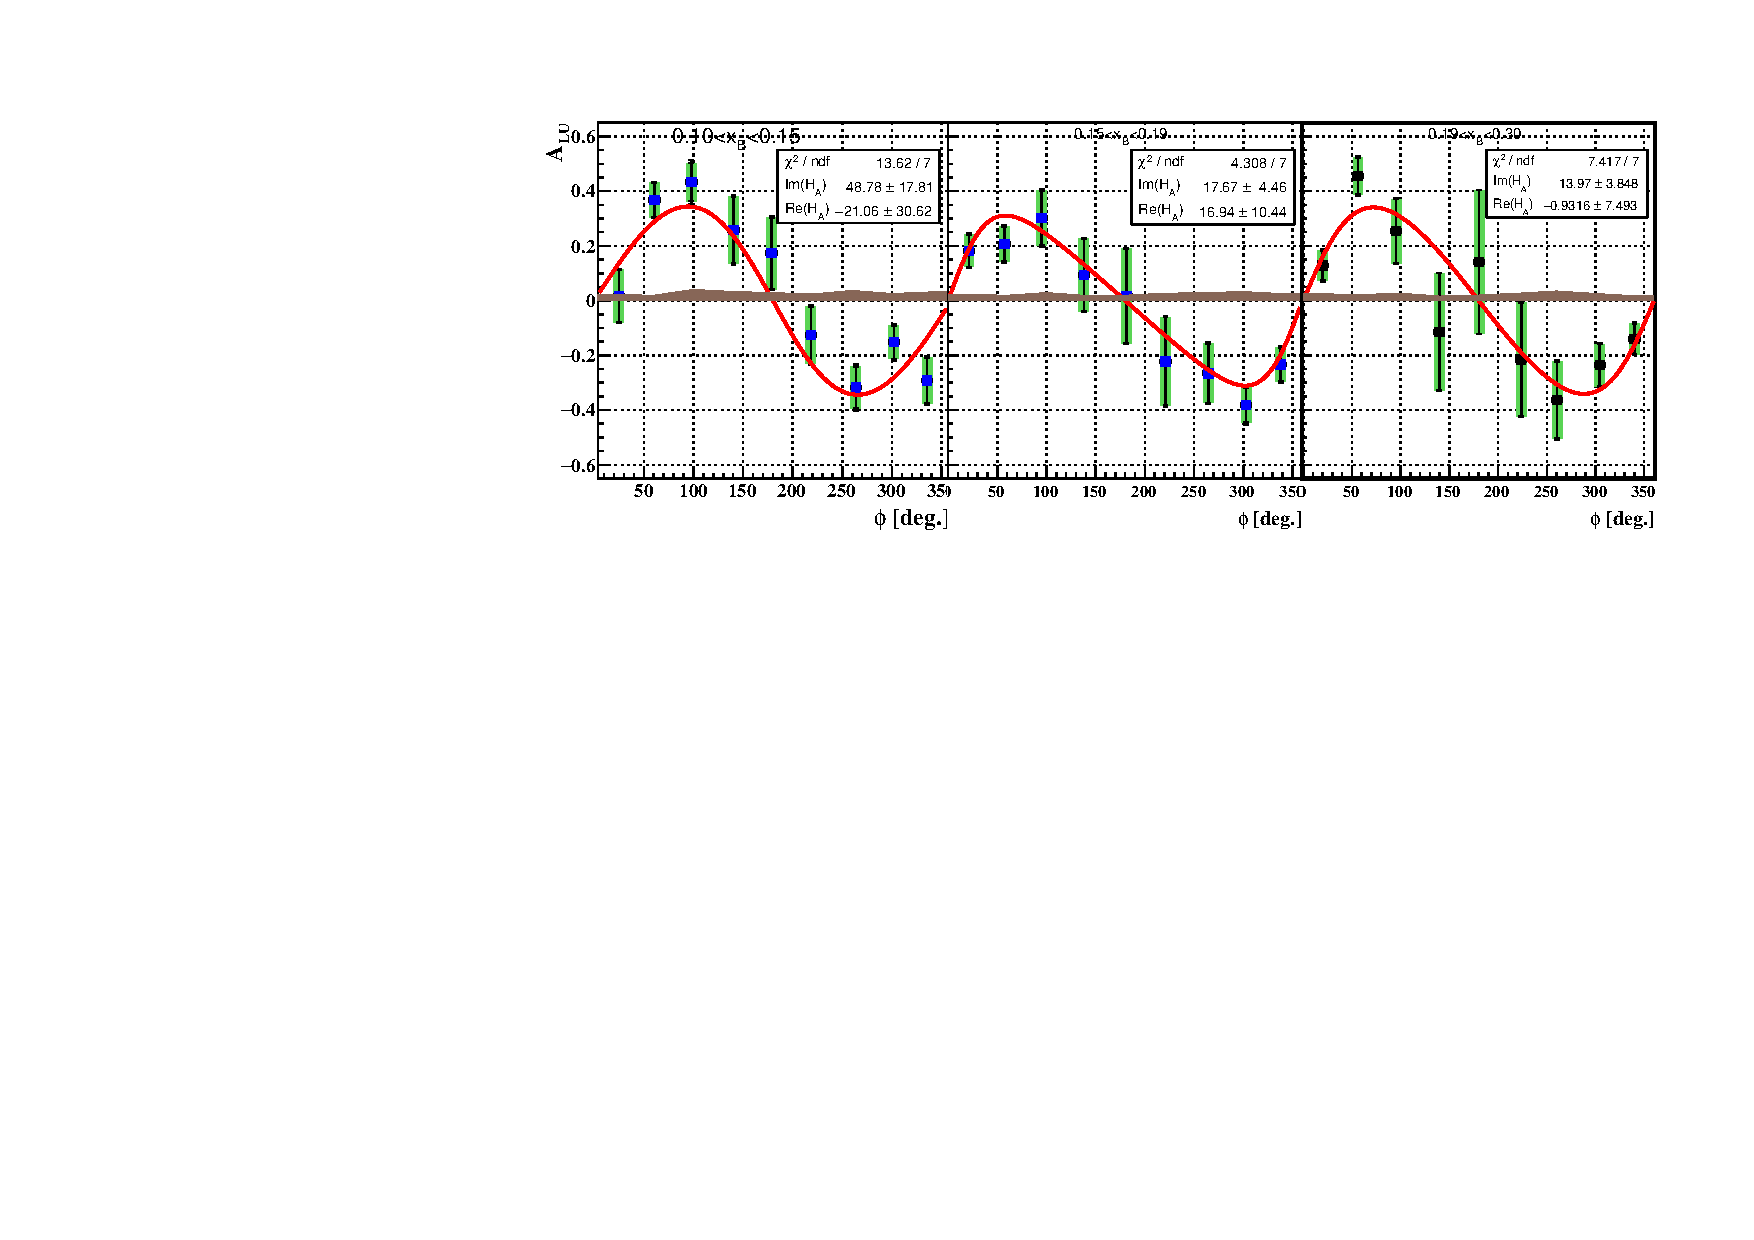
\includegraphics[height=7.5cm]{old_plots/f_coh_alu_xB_phi.pdf}
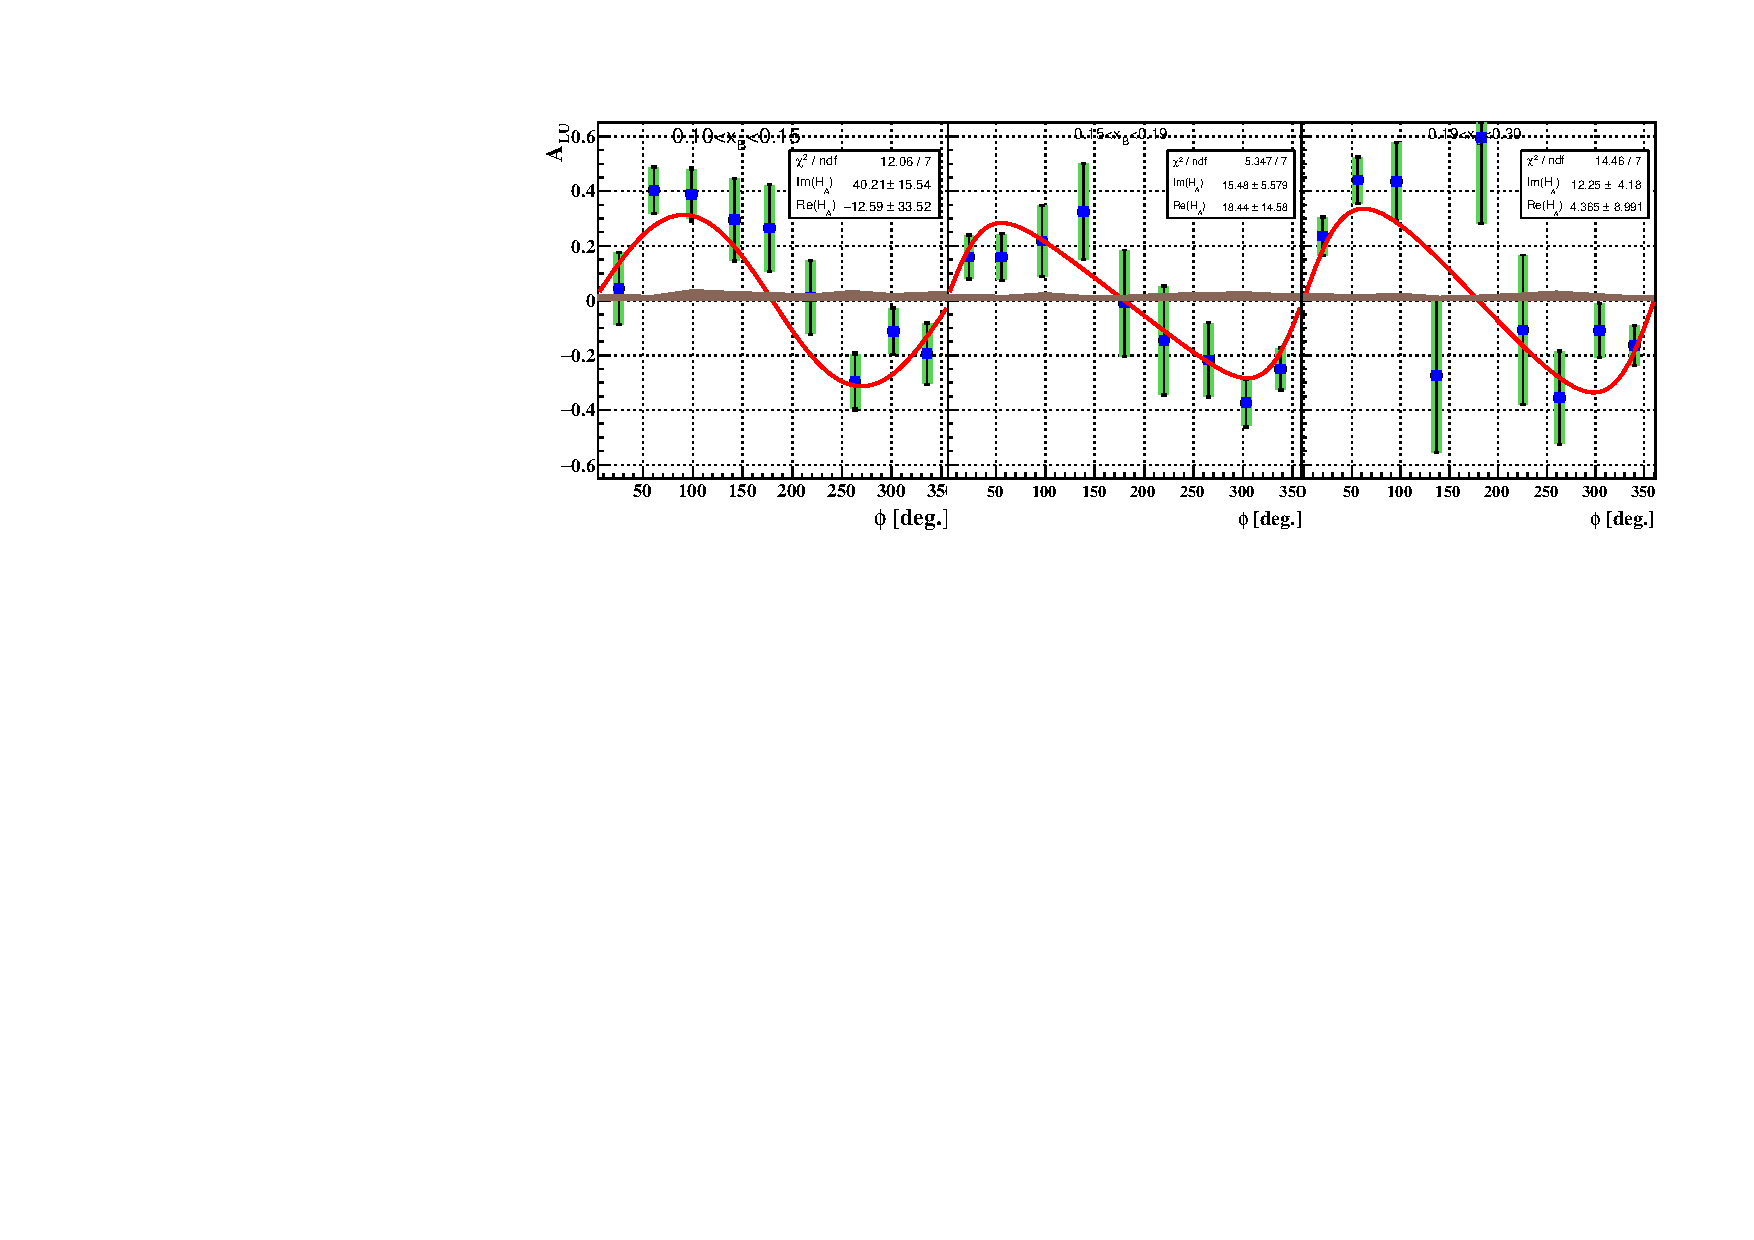
\includegraphics[height=7.5cm]{new_plots/Coh_ALU_xB_phi.pdf}
\caption{Coherent $A_{LU}$ as a function of $\phi$ in $x_{B}$ bins for old 
(top) and new (bottom) selection sets.}
\label{fig:ALU_xB_phi}
\end{figure}


\begin{figure}[h!]
\centering
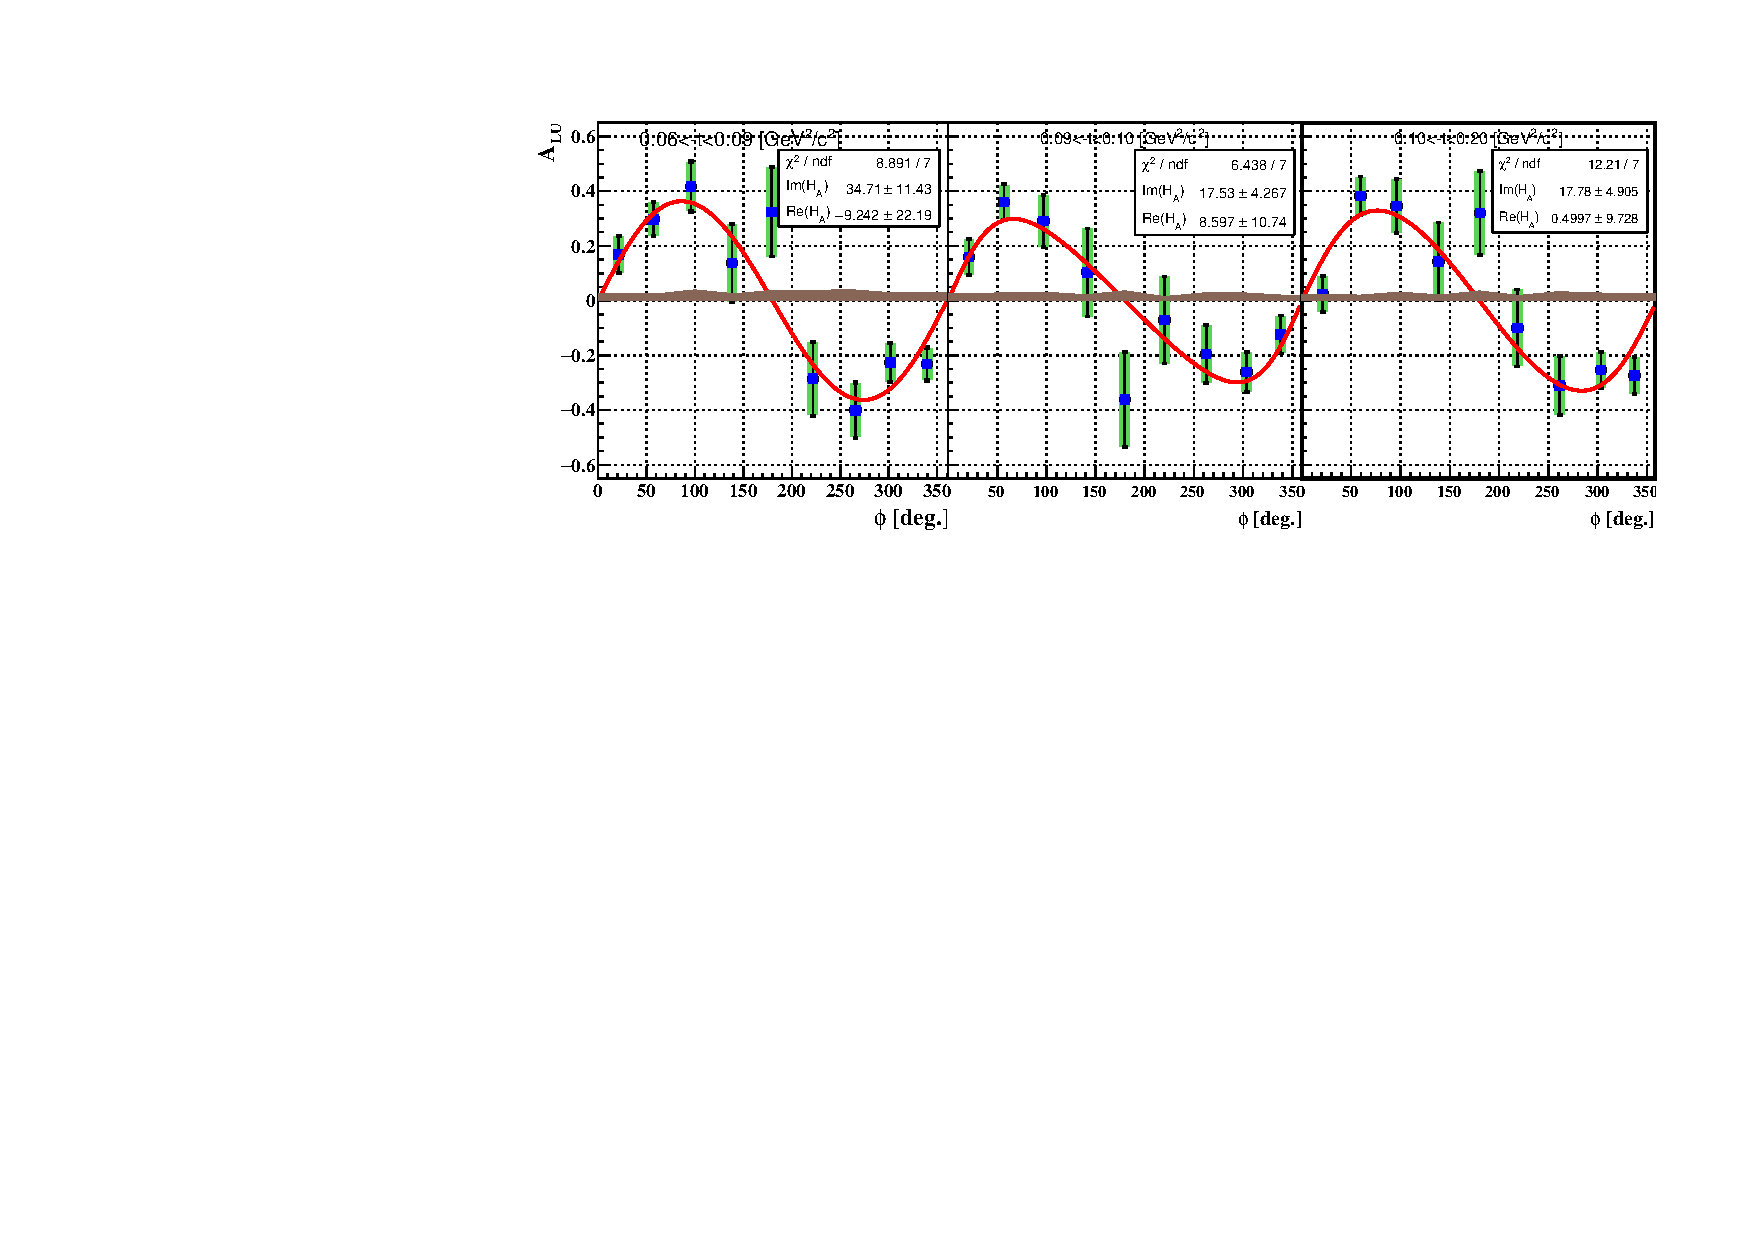
\includegraphics[height=7.5cm]{old_plots/f_coh_alu_t_phi.pdf}
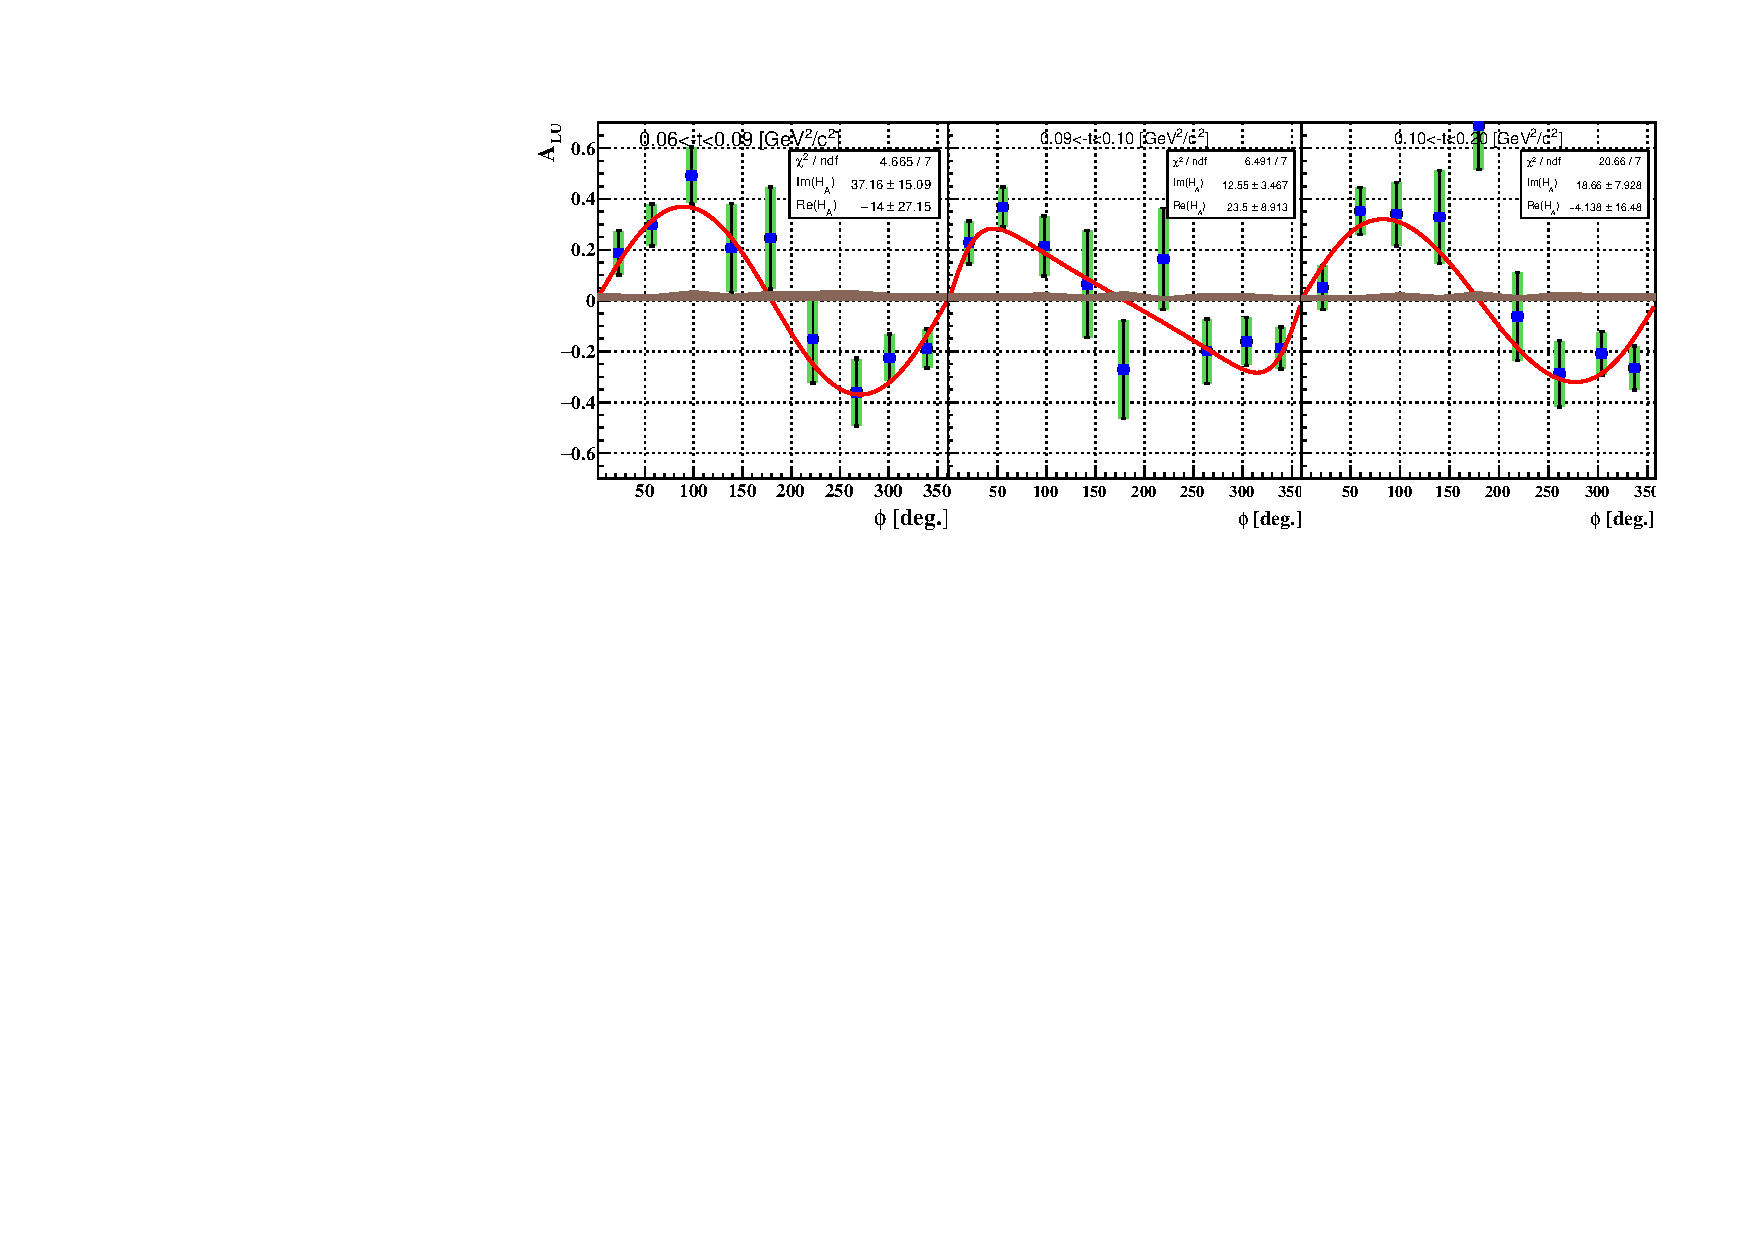
\includegraphics[height=7.5cm]{new_plots/Coh_ALU_t_phi.pdf}
\caption{Coherent $A_{LU}$ as a function of $\phi$ in $-t$ bins for old (top) 
and new (bottom) selection sets.}
\label{fig:ALU_t_phi}
\end{figure}


\begin{figure}[h!]
\centering
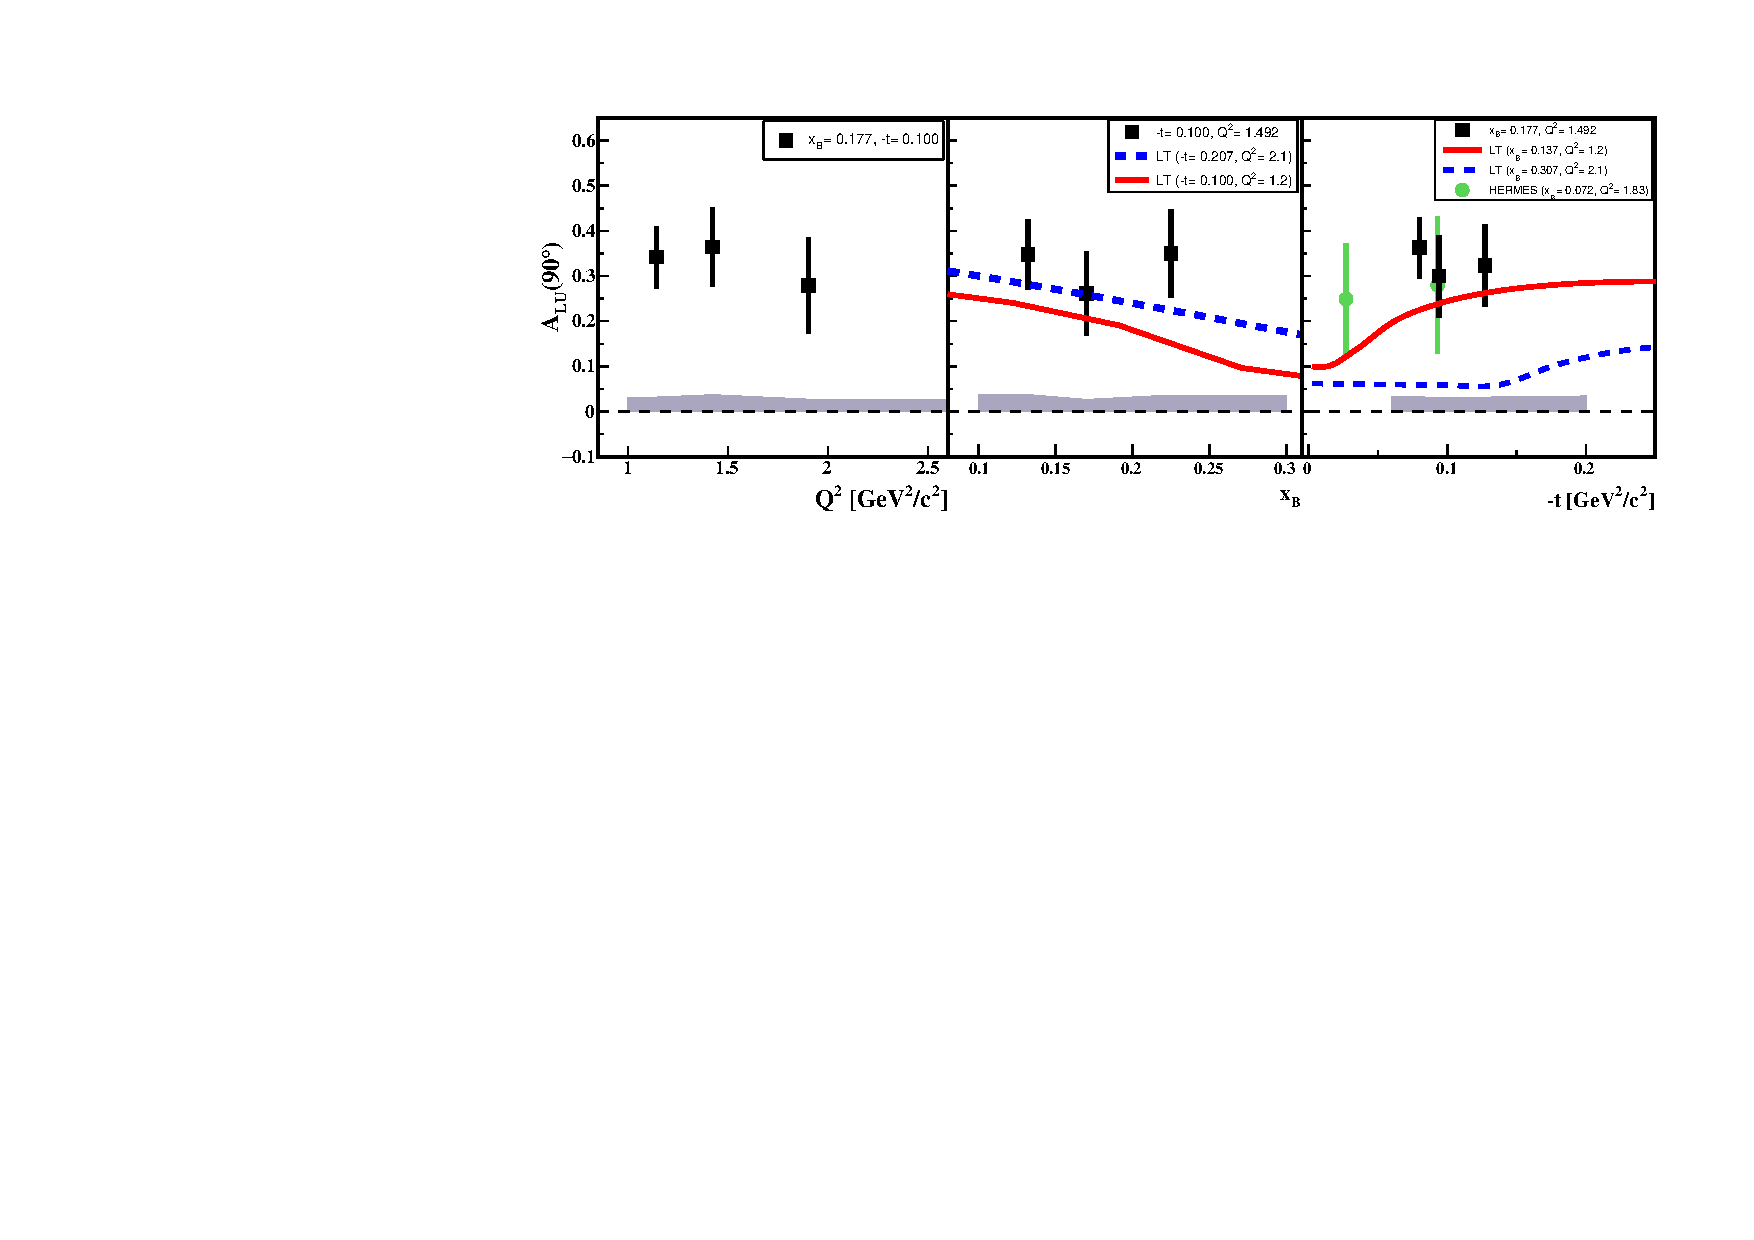
\includegraphics[height=7.0cm]{old_plots/coherent-ALU_90.pdf}
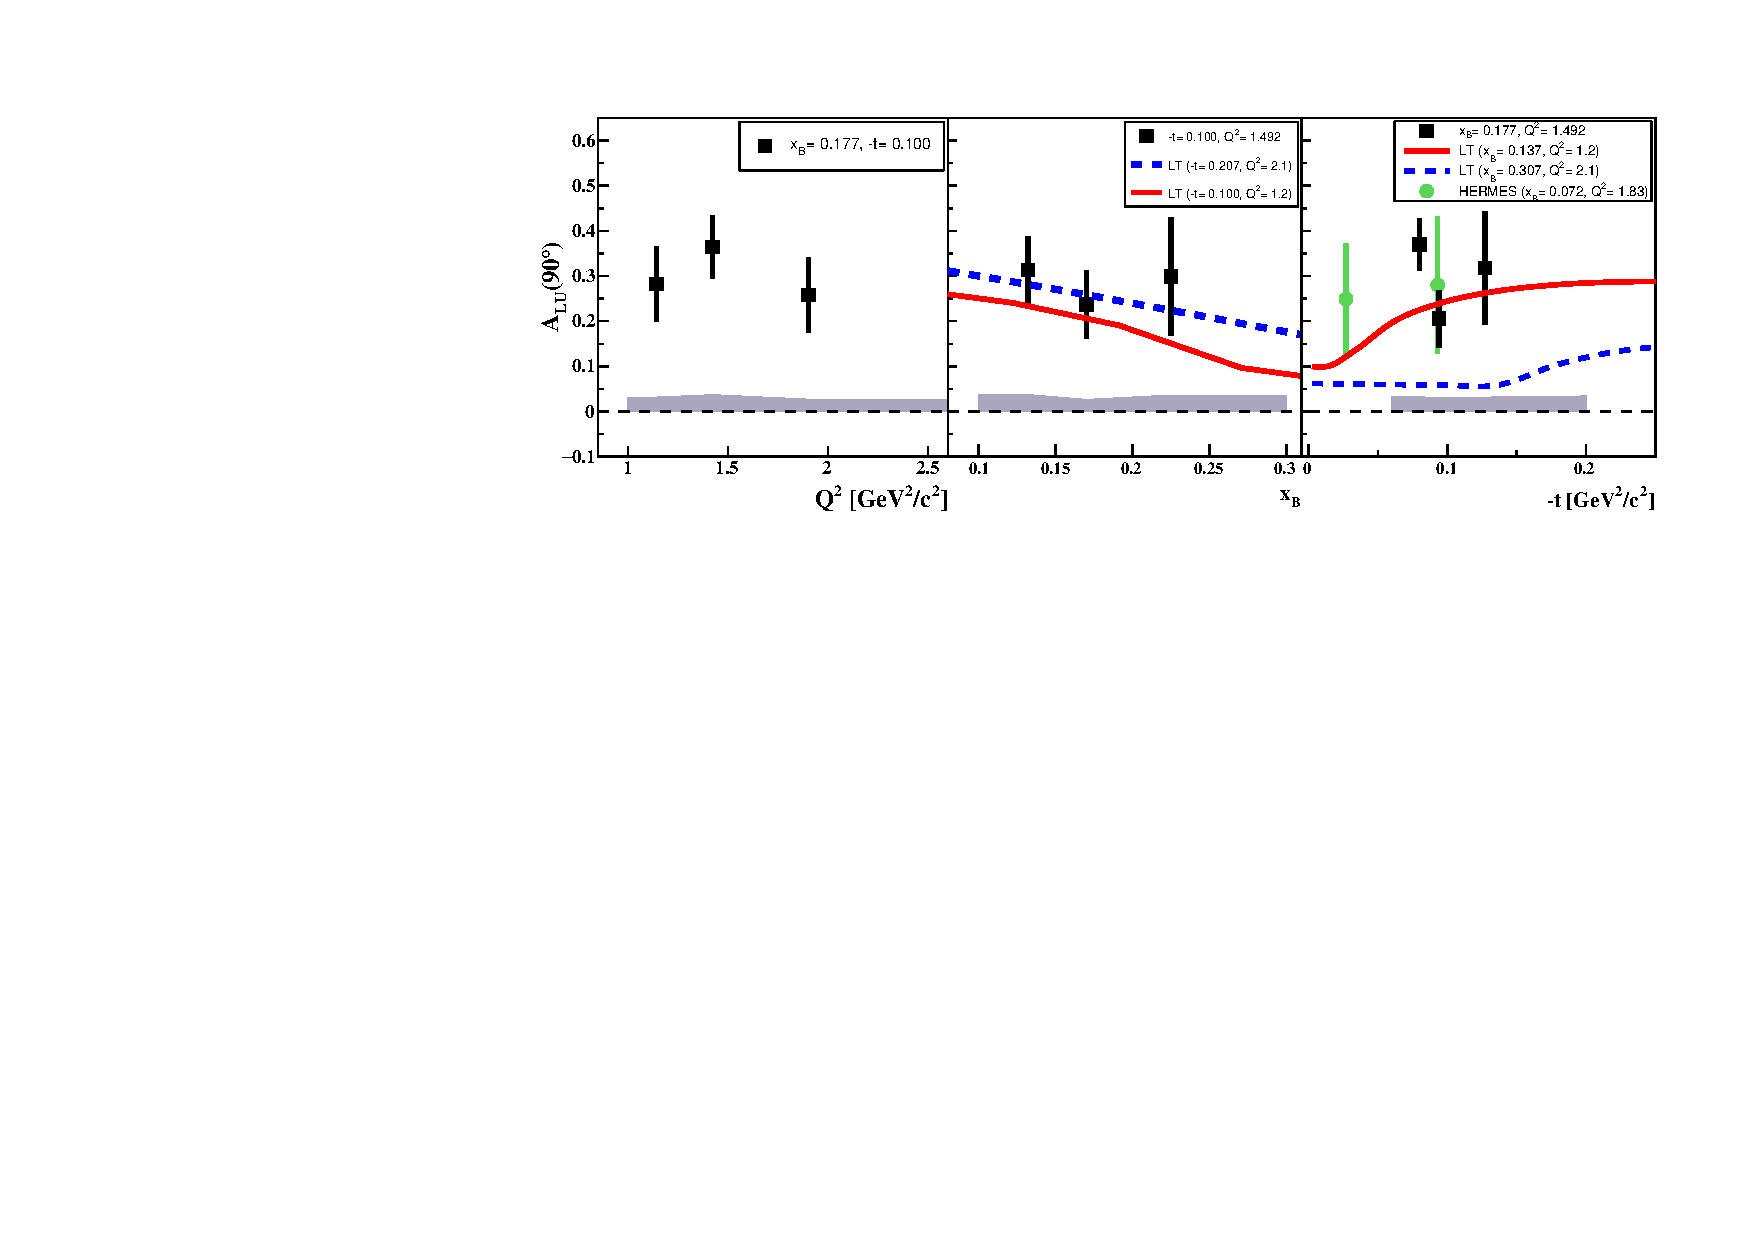
\includegraphics[height=7.0cm]{new_plots/Coh_ALU_phi_90.pdf}
\caption{Coherent $A_{LU}$ at $\phi = 90^{\circ}$ for old (top) and new 
(bottom) selection sets.}
\label{fig:ALU_90}
\end{figure}


\begin{figure}[h!]
\centering
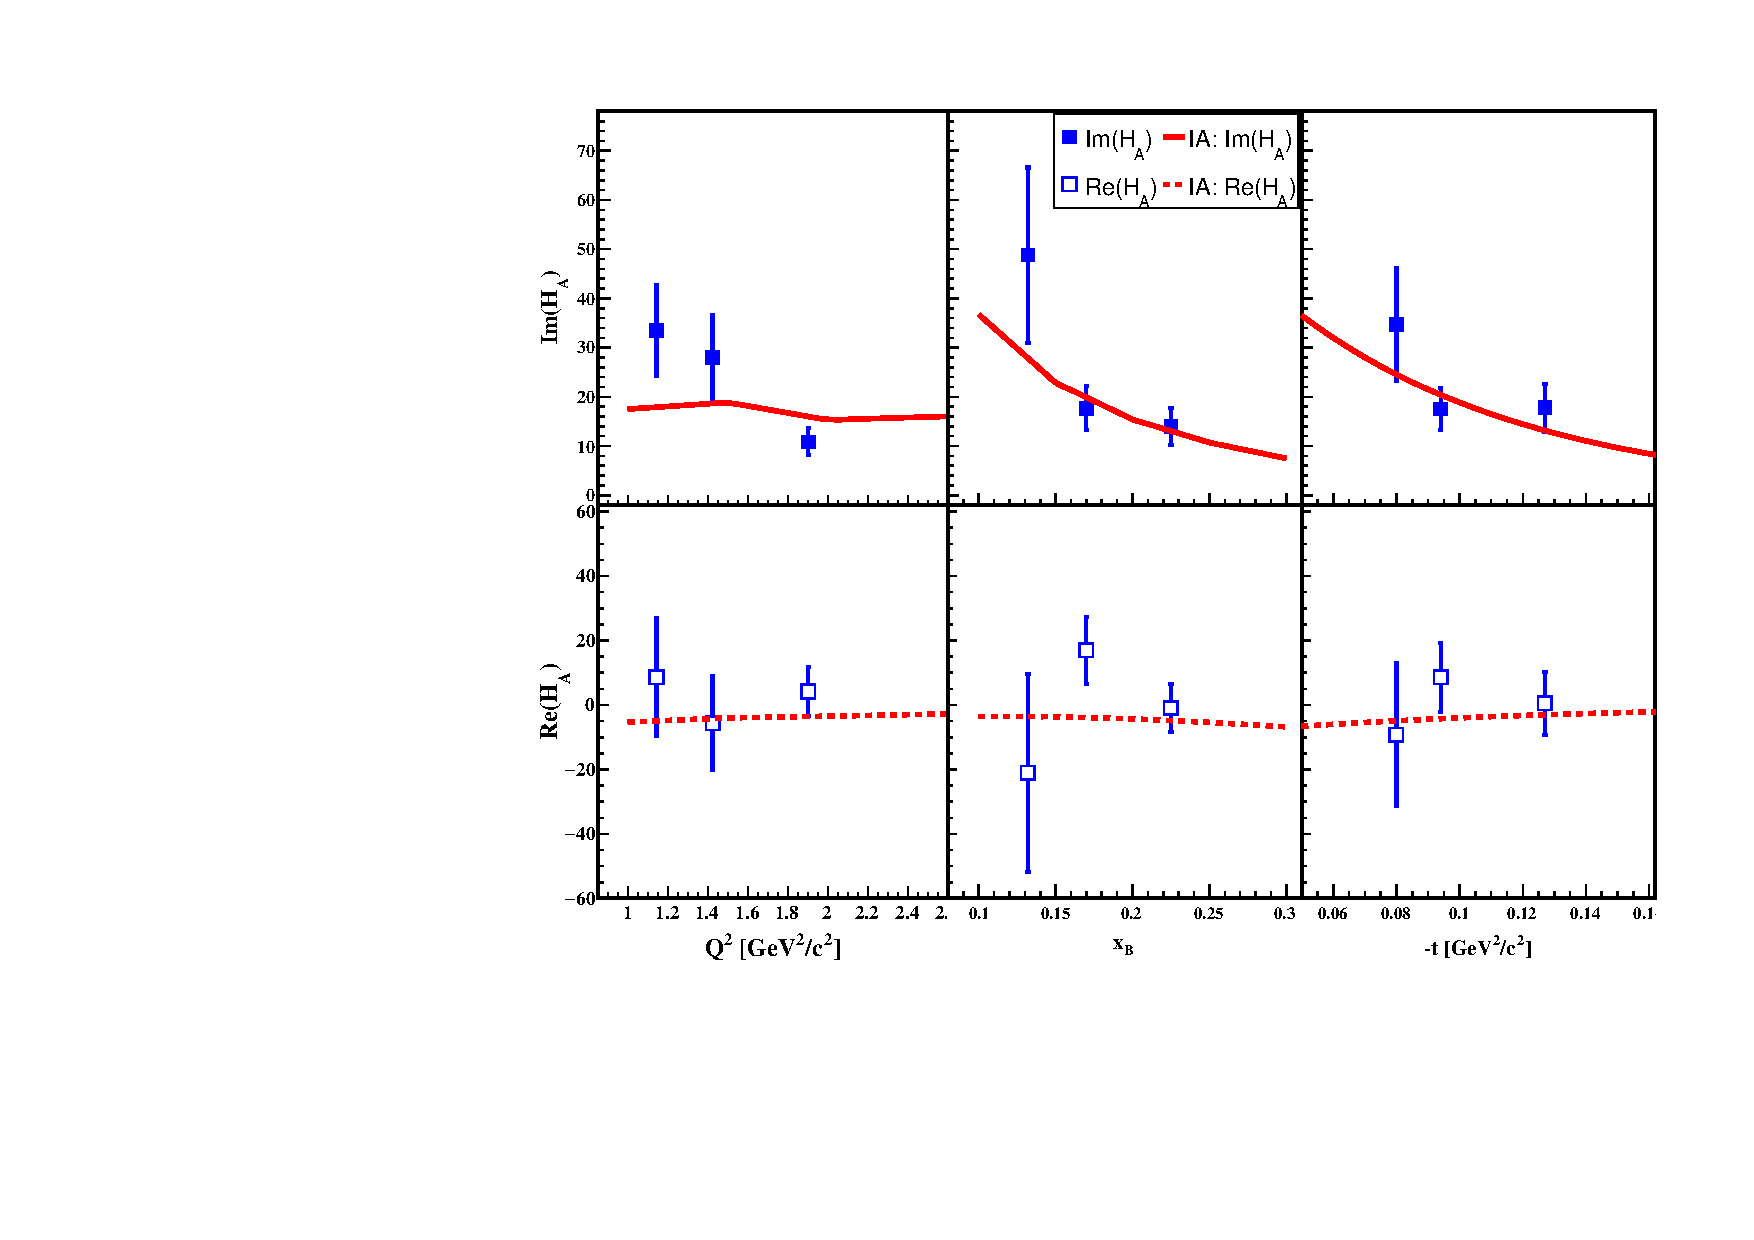
\includegraphics[height=10.0cm]{old_plots/updated_CFFs.pdf}
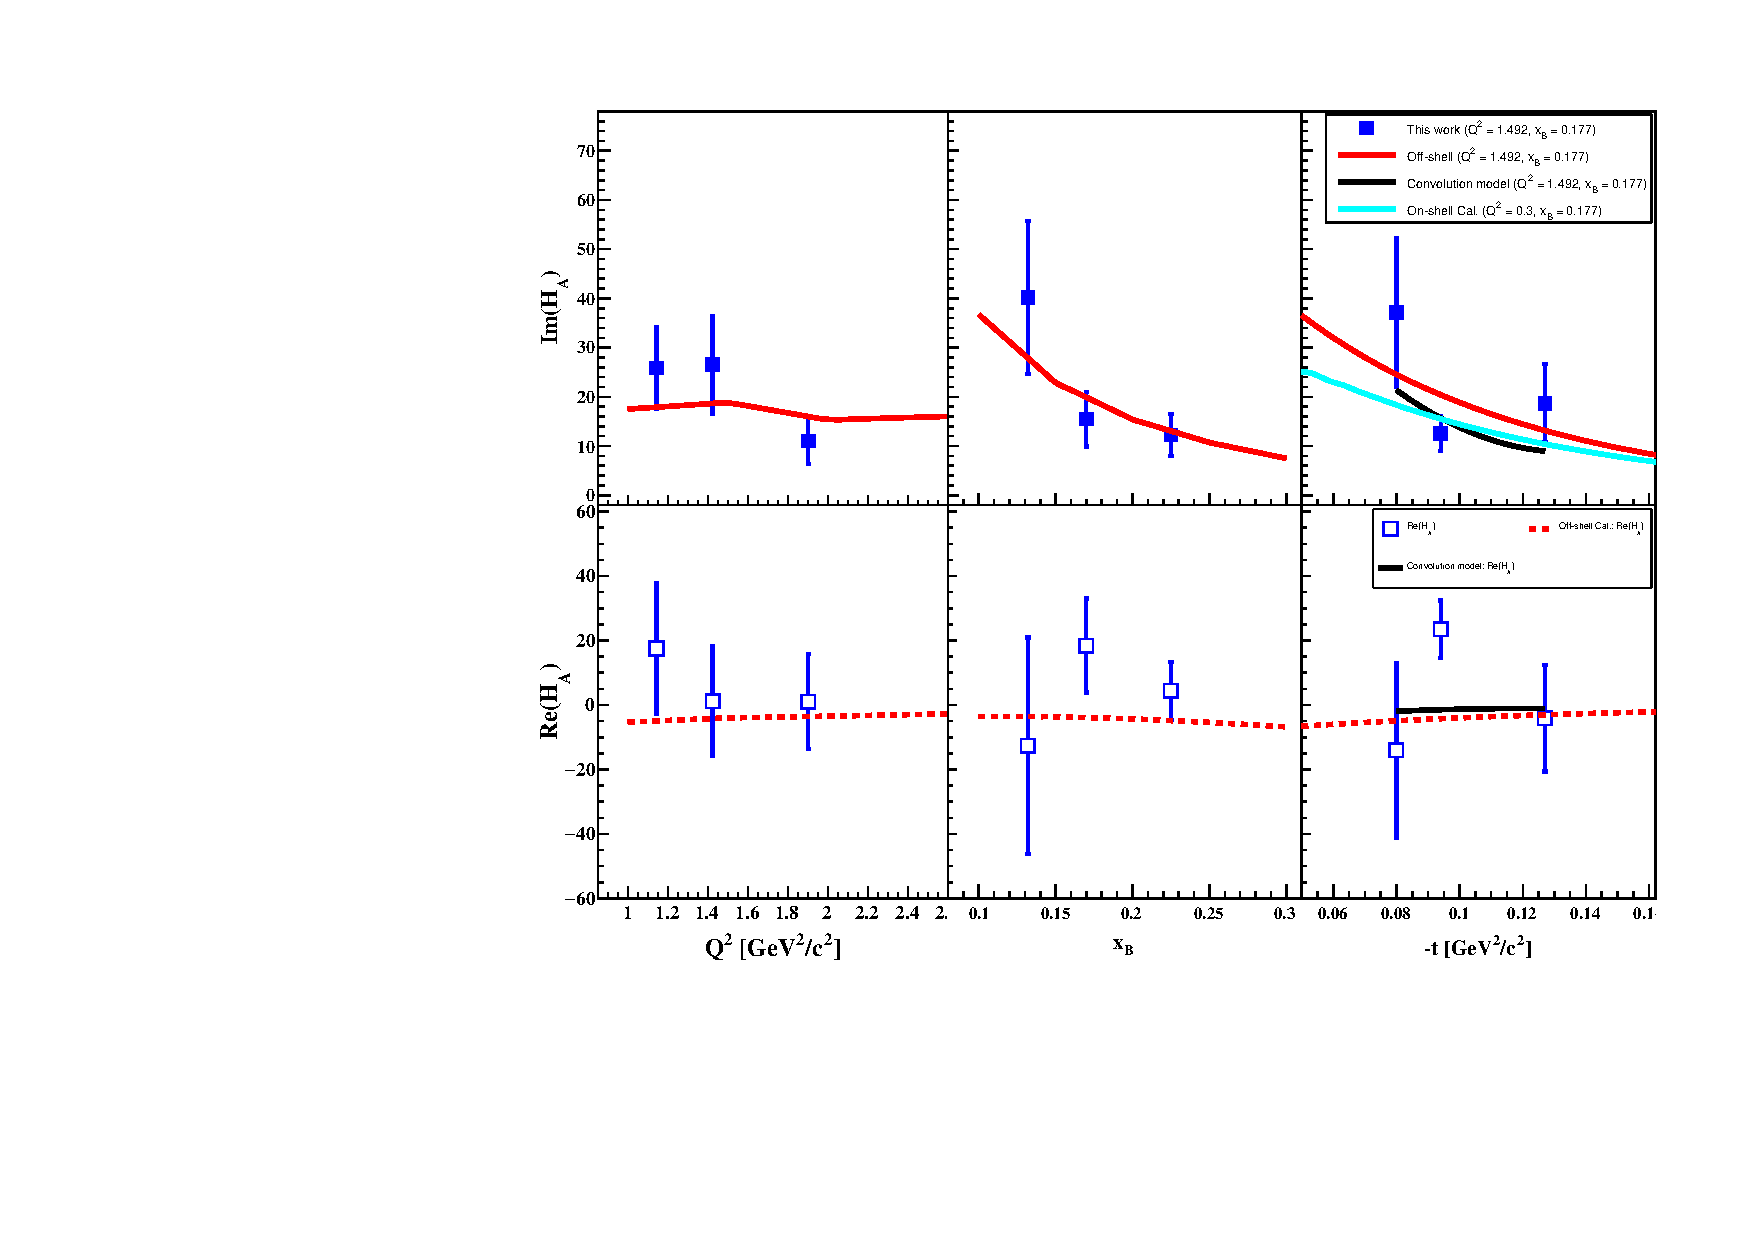
\includegraphics[height=10.0cm]{new_plots/CFF_Im_Re.pdf}
\caption{$H_{A}$ CFF from old (top) and new (bottom) selection sets.}
\label{fig:CFFs}
\end{figure}



